\chapter{Preliminary Design}

This chapter aims to provide a general overview of the design, the interaction between the different modules of the NeoPixel Sunrise Clock (NPSC). Moreover, it provides the justifications of components selection and the reasoning behind the visual design of the NPSC.

%%%%%%%%%%%%%%%%%%%%%%%%%%%%%%%%%%%%%%%%%%%%%%%%%%%%%%%%%%%%%%%%%%%%%%%%%%%%%%%%%%%%
% SECTION: System overview
%%%%%%%%%%%%%%%%%%%%%%%%%%%%%%%%%%%%%%%%%%%%%%%%%%%%%%%%%%%%%%%%%%%%%%%%%%%%%%%%%%%%
\section{System overview}
The NPSC is designed such that it is a user-friendly bedside alarm-clock serving as a supplement in the treatment of sleep-disorder via light emission. To achieve these goals, the system was designed using a modular approach. The modules illustrated in  \cref{fig:strutural_block_diagram} are the elements deemed required to achieve the goals laid out in \ref{purpose_of_the_study}. \\
The relationship between the goals defined in the introduction and these modules are given below:
\begin{itemize}
\item \textbf{Regulate the sleep-wake cycle}: This is done by emissions of specific lights parameters using the Neopixel as part of the system outputs.
\item \textbf{User-friendly}: Using push-buttons for controlling the NPSC would not be optimal it is a multifunctional device. The onboard touchscreen in the System Inputs is to remove having the users relying on push-buttons to use certain functionalities. As for the android application, it allows the users to control the devices wirelessly. Via the Android application, the NPSC has the possibility to be an Internet Of Thing (IOT) device increasing the variety of its applications.
\item \textbf{Personalisable}: The system inputs are the doors to the NPSC configurations, with both inputs being touchscreen devices, multiples functionalities can be implemented. The EEPROM is to store user-specific data such as alarm, visual preferences.
\item \textbf{Alarm-clock}: The Clock module consisting of a Real Time Clock (RTC) and an Alarm are meant to interact together to make the NPSC also an alarm clock.
\end{itemize}
\begin{figure}[ht]
\centering
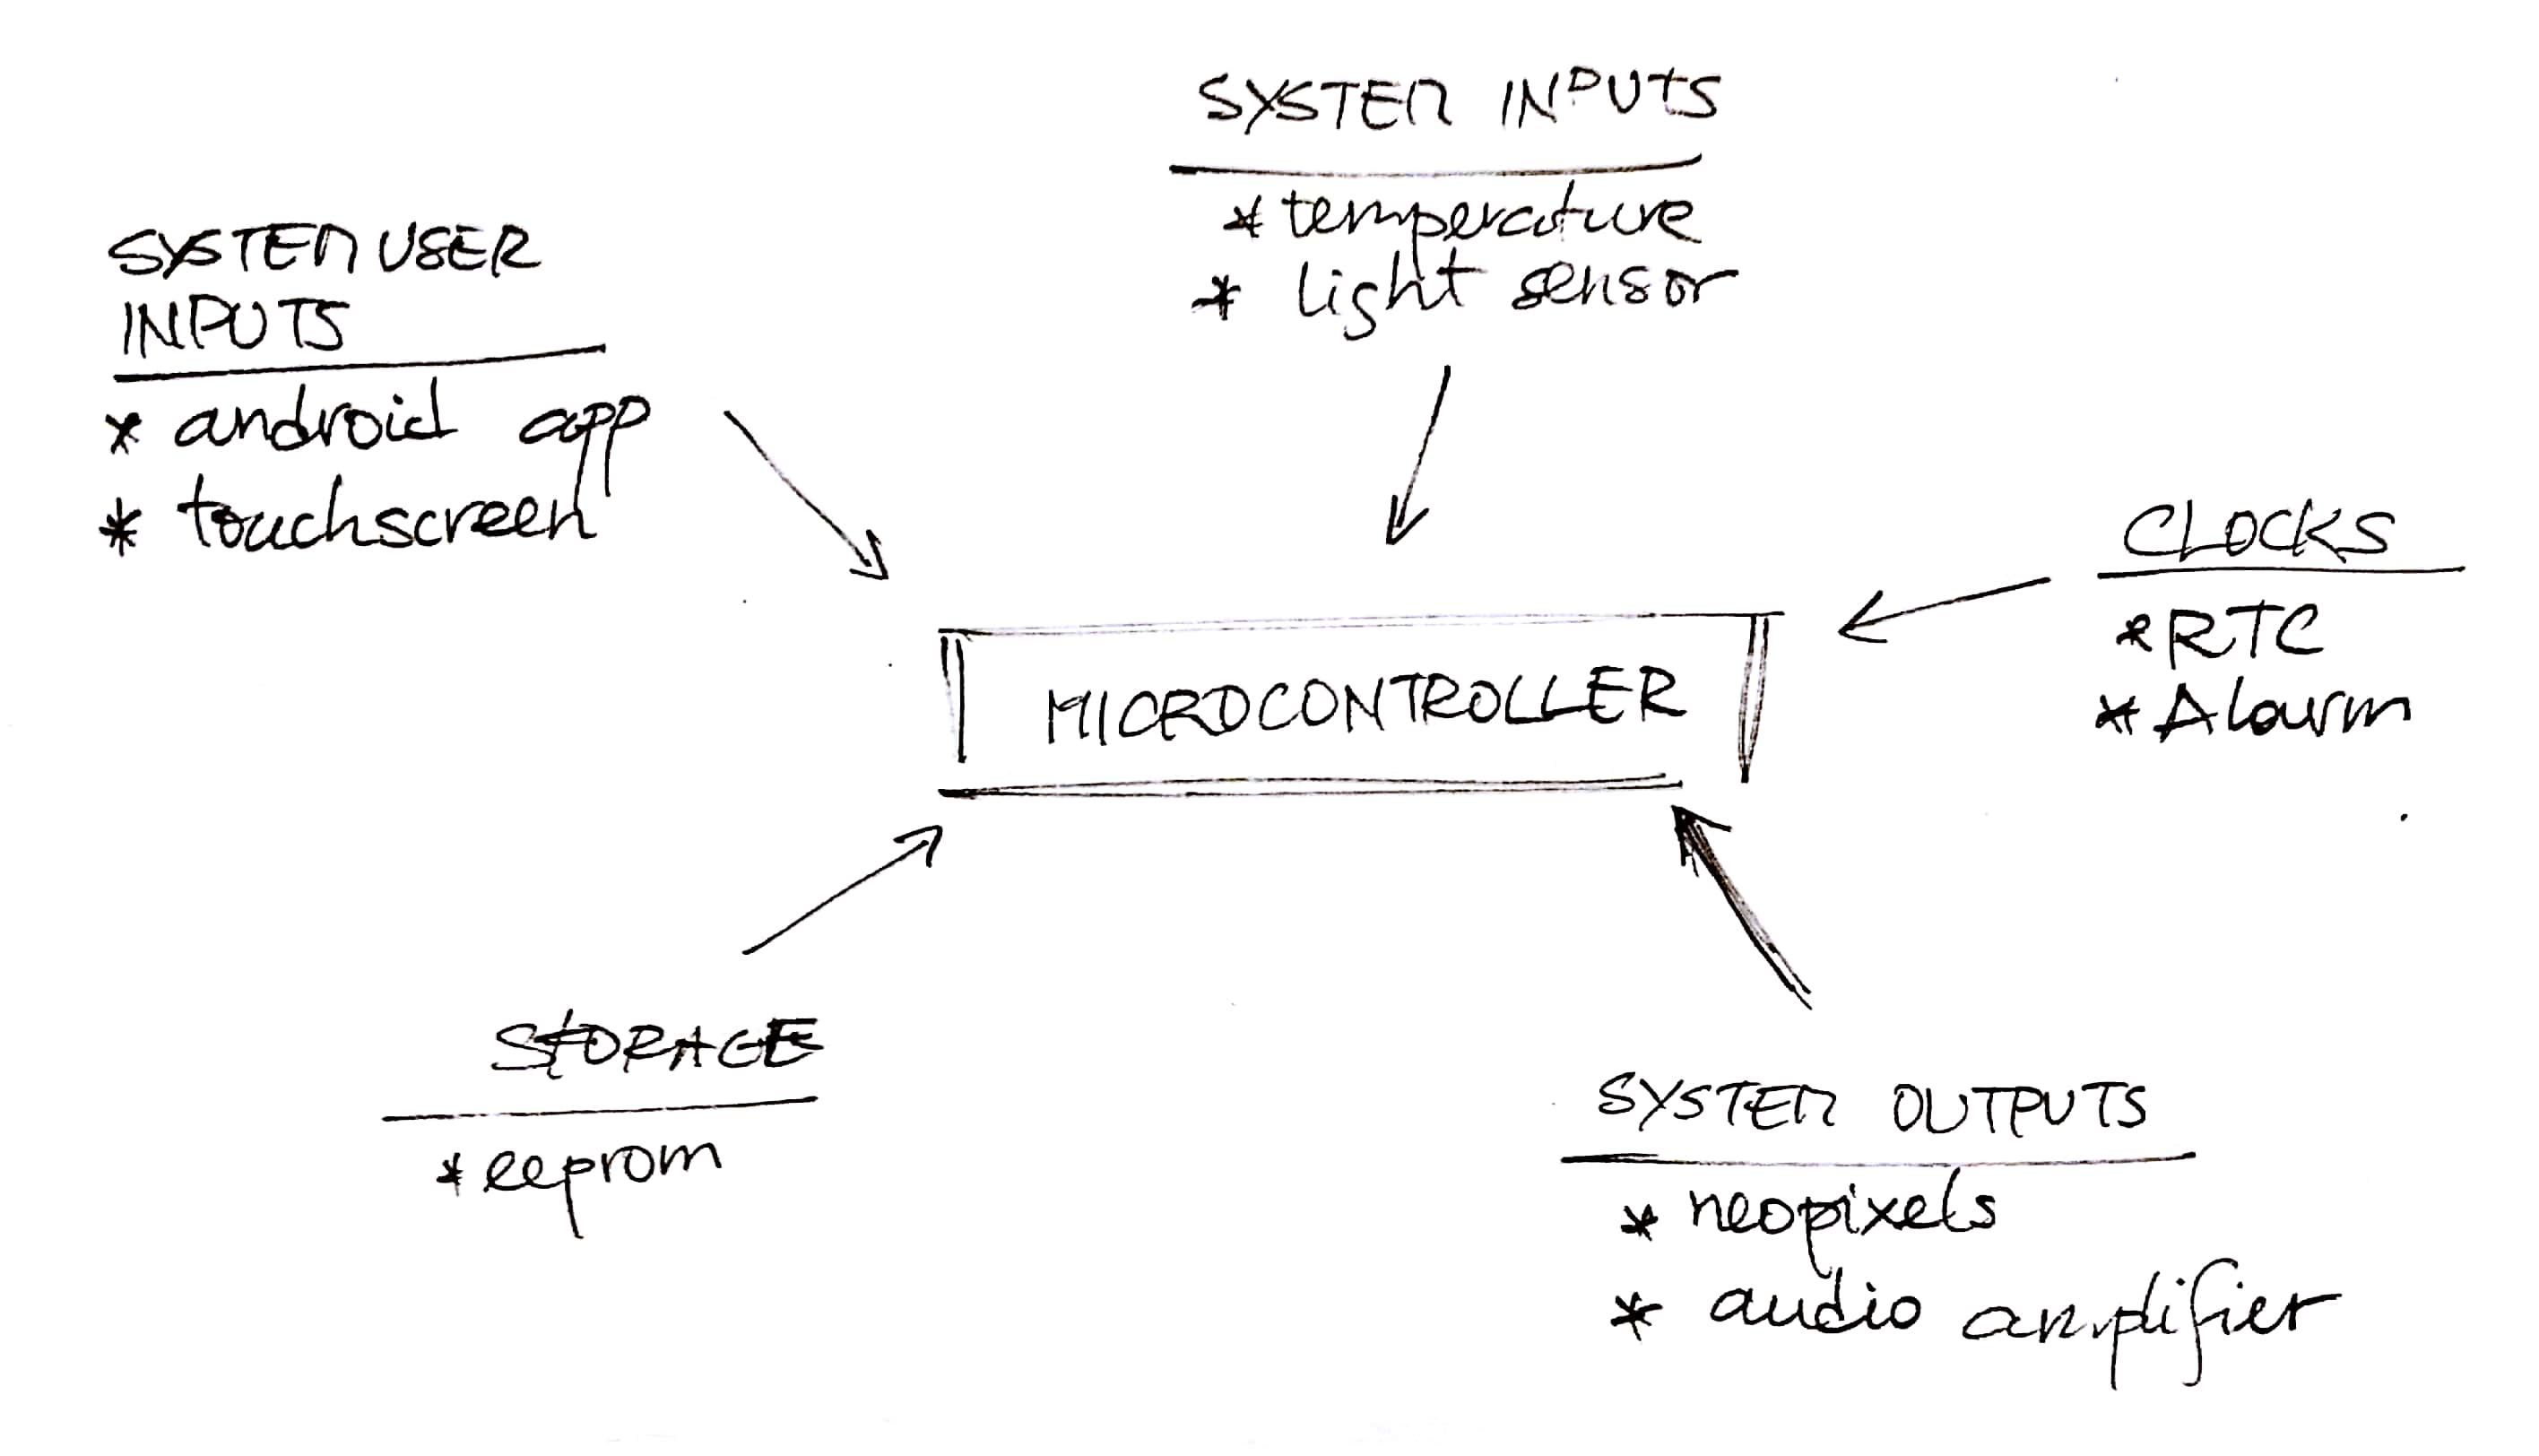
\includegraphics[scale=0.15]{strutural_block_diagram.jpg}
\caption{Structural block diagram of the NPSC.}
\label{fig:strutural_block_diagram}
\end{figure}


%%%%%%%%%%%%%%%%%%%%%%%%%%%%%%%%%%%%%%%%%%%%%%%%%%%%%%%%%%%%%%%%%%%%%%%%%%%%%%%%%%%%
% SECTION: System components selection 
%%%%%%%%%%%%%%%%%%%%%%%%%%%%%%%%%%%%%%%%%%%%%%%%%%%%%%%%%%%%%%%%%%%%%%%%%%%%%%%%%%%%
\section{System components selection}

\begin{itemize}
\item \textbf{Microcontroller}: The STM32F407VGT6 with the specifications listed in \cref{table:micro} is the one selected for the NPSC. This choice was based of its number of pins and mostly on the fact that this microcontroller has been used in previous project. 
\item \textbf{Wireless}:
\item \textbf{Eeprom}:
\item \textbf{RTC}:
\item \textbf{Light}:
\item \textbf{Touchscreen}:
\item \textbf{Android application}:
\end{itemize}

%%%%%%%%%%%%%%%%%%%%%%%%%%%%%%%%%%%%%%%%%%%%%%%%%%%%%%%%%%%%%%%%%%%%%%%%%%%%%%%%%%%%
% SECTION: Visual outputs component design decision
%%%%%%%%%%%%%%%%%%%%%%%%%%%%%%%%%%%%%%%%%%%%%%%%%%%%%%%%%%%%%%%%%%%%%%%%%%%%%%%%%%%%
\section{Visual outputs component design decisions}
Explain the need of having these components the way they are\\
Might use bullet instead of subsections
\subsection{Ring}
\subsection{Date and Temperature}
\subsection{Time}
\subsection{Weekday}
